\chapter{Uso del estilo provisto}
\chapterquote{Hablaban siempre de dinero y planeaban asaltar un banco}{Domingo Cavallo, 2001}

% Figuras de ESTE cap\'{\i}tulo + las compartidas. Siempre al principio del archivo.
\graphicspath{{figs/cap1/}{figs/comunes/}}

\section{Opciones que acepta el estilo}
\label{S:opciones-que-acepta}

\subsection*{Espaciado}
El interlineado que se utiliza en el cuerpo de la tesis es de un espacio y medio. Esto se puede cambiar usando una de las opciones
\begin{itemize}
\item Un espacio y medio, formato recomendado por el instituto (\textbf{default})
\item un s\'{o}lo espacio (\verb|\documentclass[12pt,singlespacing]{ibtesis}|) 
\item doble espacio (\verb|\documentclass[12pt,doublespacing]{ibtesis}|)
\end{itemize}

\subsection*{Formato de la p\'{a}gina}
El formato de la p\'{a}gina puede ser
\begin{itemize}
\item final Es el recomendado para la tesis por el Instituto (\textbf{default})
\item borrador (\verb|\documentclass[12pt,preprint]{ibtesis}|)\\ Es un formato con m\'{a}rgenes m\'{a}s chicos, \'{u}til para realizar correcciones en borradores 
\end{itemize}

\subsection*{Doble faz}
\label{S:doble-faz}

\begin{itemize}
\item \verb|\oneside| Los m\'{a}rgenes son iguales para todas las p\'{a}ginas
\item \verb|\twoside| P\'{a}ginas izquierdas y derechas son diferentes
\end{itemize}

\subsection*{Soporte f\'{\i}sico}

El estilo tiene una opci\'{o}n para soporte en papel y en pantalla:
\begin{itemize}
\item En papel (\verb|\documentclass[12pt,paper]{ibtesis}|) (\textbf{default})
\item En pantalla (archivo pdf) (\verb|\documentclass[12pt,screen]{ibtesis}|)\\
Incluye links y algunos colores en el texto
\end{itemize}

\subsection*{Otras opciones}
\label{S:otras-opciones}
Otras opciones con las que se cargue el estilo se pasan directamente a los estilos usados. Por ejemplo si usamos:\\
\verb|\documentclass[11pt,screen,oneside,preprint,draft,pagebackref]{ibtesis}|\\
producir\'{a} un documento con letra de menor tama\~{n}o (11pt), no se procesar\'{a}n los gr\'{a}ficos (draft) para una mayor velocidad, se producir\'{a}n links en el archivo pdf con la caracter\'{\i}stica adicional que las referencias tendr\'{a}n un link al lugar donde fueron citadas ya que la opci\'{o}n \verb|pagebackref| se pasa al paquete \verb|\hyperref|.

\section{Par\'{a}metros convenientes}
\label{S:param-conv}

Se han definido tres longitudes que pueden servir para dar un ancho uniforme a todas las figuras.
Estas longitudes se han definido s\'{o}lo por conveniencia. 

Los valores que se le han dado son:
\begin{itemize}
\item \verb|\imsize= 0.7\textwidth|
\item \verb|\imsizeS= 0.5\textwidth|
\item \verb|\imsizeL= 0.9\textwidth|
\end{itemize}

Si se quieren modificar, puede hacerse usando el comando \verb|\setlength|, por ejemplo:
\begin{itemize}
\item \verb|\setlength{\imsizeL}{0.85\textwidth}|
\item \verb|\setlength{\imsize}{3.6in}|
\item \verb|\setlength{\imsizeS}{8.6cm}|
\end{itemize}

\section{Figuras}
\label{S:figuras}

La figura se busca en las carpetas declaradas en \verb|\graphicspath| al
principio de este archivo, en orden. Por eso en el \verb|\includegraphics| va
s\'{o}lo el nombre del archivo, sin la carpeta.

\begin{figure}[ht]
\centering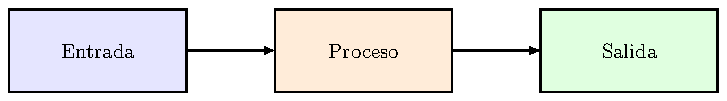
\includegraphics[width=\imsize]{cap1_esquema}
\caption[Esquema de bloques]{Esta figura vive en \texttt{figs/cap1/}.
\label{f:cap1-esquema}}
\end{figure}

\begin{figure}[ht]
\centering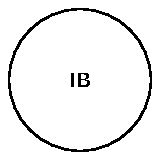
\includegraphics[width=\imsizeS]{logo_ib}
\caption[Figura compartida]{Esta otra vive en \texttt{figs/comunes/} y la puede
usar cualquier cap\'{\i}tulo.\label{f:cap1-logo}}
\end{figure}

\section{Citas}
\label{S:citas}

Cita simple \cite{Bohm1952PRp166}. Cita m\'{u}ltiple, que el estilo comprime:
\cite{Bohm1952PRp166,Bohm1952PRp180,Bohr1913PMp10}.

Cita a una p\'{a}gina puntual: \cite[172]{Bohm1952PRp166}. Si el localizador es un
n\'{u}mero pelado, biblatex le pone \'{e}l mismo el prefijo correcto (singular o
plural seg\'{u}n sea p\'{a}gina o rango): \cite[180-185]{Bohm1952PRp180}.

Cita a un cap\'{\i}tulo de un libro ya citado: \citecap{Sakurai2011}{5}, y a una
secci\'{o}n: \citesec{Sakurai2011}{5.3}.

Una referencia que es en s\'{\i} un cap\'{\i}tulo de libro se carga como
\verb|@incollection| o \verb|@inbook| y se cita normal:
\cite{Briggs1991AAMOP_TTOp1}.

Estilo autor-a\~{n}o cuando hace falta nombrar al autor en la oraci\'{o}n:
seg\'{u}n \textcite{Bohm1952PRp166} la teor\'{\i}a admite variables ocultas.

% Bibliograf\'{\i}a de este cap\'{\i}tulo. Va al final del archivo, siempre.
\bibliografiacapitulo

%%% Local Variables:
%%% mode: latex
%%% TeX-master: "template"
%%% End: 
